% Options for packages loaded elsewhere
\PassOptionsToPackage{unicode}{hyperref}
\PassOptionsToPackage{hyphens}{url}
%
\documentclass[
]{article}
\usepackage{amsmath,amssymb}
\usepackage{iftex}
\ifPDFTeX
  \usepackage[T1]{fontenc}
  \usepackage[utf8]{inputenc}
  \usepackage{textcomp} % provide euro and other symbols
\else % if luatex or xetex
  \usepackage{unicode-math} % this also loads fontspec
  \defaultfontfeatures{Scale=MatchLowercase}
  \defaultfontfeatures[\rmfamily]{Ligatures=TeX,Scale=1}
\fi
\usepackage{lmodern}
\ifPDFTeX\else
  % xetex/luatex font selection
\fi
% Use upquote if available, for straight quotes in verbatim environments
\IfFileExists{upquote.sty}{\usepackage{upquote}}{}
\IfFileExists{microtype.sty}{% use microtype if available
  \usepackage[]{microtype}
  \UseMicrotypeSet[protrusion]{basicmath} % disable protrusion for tt fonts
}{}
\makeatletter
\@ifundefined{KOMAClassName}{% if non-KOMA class
  \IfFileExists{parskip.sty}{%
    \usepackage{parskip}
  }{% else
    \setlength{\parindent}{0pt}
    \setlength{\parskip}{6pt plus 2pt minus 1pt}}
}{% if KOMA class
  \KOMAoptions{parskip=half}}
\makeatother
\usepackage{xcolor}
\usepackage[margin=1in]{geometry}
\usepackage{graphicx}
\makeatletter
\def\maxwidth{\ifdim\Gin@nat@width>\linewidth\linewidth\else\Gin@nat@width\fi}
\def\maxheight{\ifdim\Gin@nat@height>\textheight\textheight\else\Gin@nat@height\fi}
\makeatother
% Scale images if necessary, so that they will not overflow the page
% margins by default, and it is still possible to overwrite the defaults
% using explicit options in \includegraphics[width, height, ...]{}
\setkeys{Gin}{width=\maxwidth,height=\maxheight,keepaspectratio}
% Set default figure placement to htbp
\makeatletter
\def\fps@figure{htbp}
\makeatother
\setlength{\emergencystretch}{3em} % prevent overfull lines
\providecommand{\tightlist}{%
  \setlength{\itemsep}{0pt}\setlength{\parskip}{0pt}}
\setcounter{secnumdepth}{-\maxdimen} % remove section numbering

\usepackage[utf8]{inputenc}
\usepackage[T1]{fontenc}
%\usepackage[french]{babel}
\usepackage{graphicx}
\usepackage{fullpage}
\usepackage{eso-pic}

%%% BLOQUER LES PLOTS
\usepackage{float}
\let\origfigure\figure
\let\endorigfigure\endfigure
\renewenvironment{figure}[1][2]{
    \expandafter\origfigure\expandafter[H]
} {
    \endorigfigure
}


\newcommand{\HRule}{\rule{\linewidth}{0.5mm}}
\newcommand{\blap}[1]{\vbox to 0pt{#1\vss}}
\newcommand\AtUpperLeftCorner[3]{%
  \put(\LenToUnit{#1},\LenToUnit{\dimexpr\paperheight-#2}){\blap{#3}}%
}
\newcommand\AtUpperRightCorner[3]{%
  \put(\LenToUnit{\dimexpr\paperwidth-#1},\LenToUnit{\dimexpr\paperheight-#2}){\blap{\llap{#3}}}%
}


\title{\Huge{Rapport sur le modèle de mélange}}
\author{\Large{Projet tutoré}}
\makeatletter

\AtBeginDocument{
\begin{titlepage}
    \enlargethispage{2cm}

    \AddToShipoutPicture{
        \AtUpperLeftCorner{1.5cm}{1cm}{
\includegraphics[width=5cm]{logoIM2AG.png}}
        \AtUpperLeftCorner{9cm}{1cm}{
\includegraphics[width=3cm]{logoLJK.png}}
        \AtUpperLeftCorner{6.5cm}{15cm}{
\includegraphics[width=9cm]{logoUT4M.jpeg}}
        \AtUpperRightCorner{1.5cm}{1cm}{
\includegraphics[width=5cm]{logoSENS.png}}
        }

    \begin{center}
        \vspace*{8cm}
        \textsc{\@title}
        \HRule
        \vspace*{0.5cm}
        \Large{Projet tutoré}
    \end{center}

    \vspace*{10cm}

 \par\noindent\rlap{\Large Océane Baboulaz, Alice Chauveau}\hfill\llap{\Large M2 SSD}\par
 \par\noindent\rlap{\Large Charline Champ et Morgane Maulet}\hfill\llap{\Large Année universitaire 2023/2024}\par
\end{titlepage}
\ClearShipoutPicture

}
\usepackage{booktabs}
\usepackage{caption}
\usepackage{longtable}
\usepackage{colortbl}
\usepackage{array}
\ifLuaTeX
  \usepackage{selnolig}  % disable illegal ligatures
\fi
\IfFileExists{bookmark.sty}{\usepackage{bookmark}}{\usepackage{hyperref}}
\IfFileExists{xurl.sty}{\usepackage{xurl}}{} % add URL line breaks if available
\urlstyle{same}
\hypersetup{
  hidelinks,
  pdfcreator={LaTeX via pandoc}}

\author{}
\date{\vspace{-2.5em}}

\begin{document}

\newpage
\tableofcontents

\newpage

\hypertarget{introduction}{%
\section{Introduction}\label{introduction}}

Dans cette étude, nous explorons les nuances psychologiques des coureurs
de trail en utilisant des techniques de clustering pour identifier des
groupes homogènes au sein de cette communauté. L'objectif principal est
d'analyser les profils distincts émergents au sein de cette population
hétérogène, en mettant l'accent sur les caractéristiques individuelles
telles que la motivation, l'anxiété, les habitudes de vie et d'autres
aspects psychologiques.

À travers une approche méthodologique basée sur le clustering gaussien
implémentée avec le package \emph{mclust} en \(R\), cette étude cherche
à déterminer le nombre optimal de groupes représentatifs des coureurs de
trail. Une fois ces groupes identifiés, nous nous pencherons sur les
différences significatives entre eux, afin de mieux comprendre les
dynamiques psychologiques et comportementales qui sous-tendent la
passion commune du trail running.

\newpage

\hypertarget{moduxe9lisation-par-clustering-mclust}{%
\section{Modélisation par clustering
(mclust)}\label{moduxe9lisation-par-clustering-mclust}}

Nous avons élaboré divers modèles de mélanges afin d'explorer nos
données. Pour simplifier, un modèle de mélange est un outil qui nous
guide pour déceler différents groupes ou composants au sein de nos
informations, ce qui peut être précieux pour dévoiler des schémas ou des
tendances dissimulées. Pour choisir le modèle le plus adapté, nous avons
ajusté la variable ``G'' de 1 à 5, en observant la meilleure valeur du
BIC, nous permettant ainsi de sélectionner notre modèle optimal.

\begin{figure}
\centering
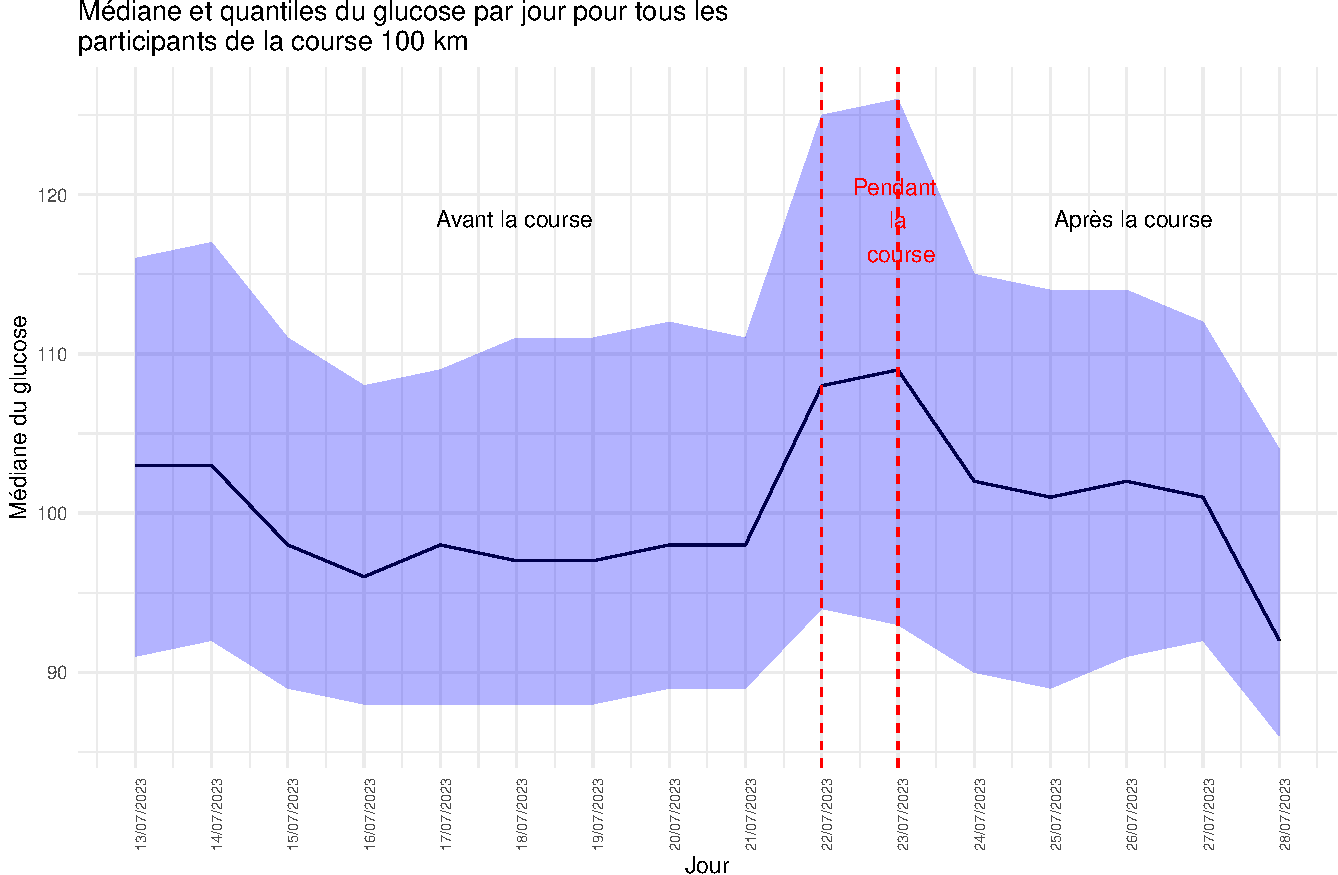
\includegraphics{Modèle_mélange_files/figure-latex/unnamed-chunk-2-1.pdf}
\caption{Comparaison des valeurs BIC pour différents modèles}
\end{figure}

Nous avons choisi le modèle de clustering avec deux groupes, car il a la
meilleure valeur du BIC (Bayesian Information Criterion). Cela suggère
qu'il correspond le mieux à la structure sous-jacente des données des
coureurs de trail.

\newpage

\hypertarget{attribution-des-clusters-aux-donnuxe9es}{%
\section{Attribution des clusters aux
données}\label{attribution-des-clusters-aux-donnuxe9es}}

Voici la sortie générée par R, nous permettant d'examiner notre modèle
choisi. Le code suivant a été utilisé pour créer le modèle et afficher
ses caractéristiques :

\begin{verbatim}
> ---------------------------------------------------- 
> Gaussian finite mixture model fitted by EM algorithm 
> ---------------------------------------------------- 
> 
> Mclust VVI (diagonal, varying volume and shape) model with 2 components: 
> 
>  log-likelihood   n df      BIC      ICL
>        3277.124 320 81 6087.015 6058.658
> 
> Clustering table:
>   1   2 
> 189 131
\end{verbatim}

Ce morceau de code ajuste un modèle de mélange gaussien avec deux
groupes (G=2) en utilisant les données spécifiées. Ensuite, la fonction
summary() nous fournit un aperçu détaillé des résultats du modèle. Cela
inclut des informations telles que les paramètres estimés pour chaque
groupe, les proportions de chaque groupe, et d'autres mesures
importantes liées à la qualité du modèle. L'analyse de cette sortie nous
permet de mieux comprendre la structure de nos données et les
caractéristiques de chaque groupe identifié.

Incorporons les classifications des clusters dans notre dataframe
initial. Pour ensuite afficher les premières lignes du dataframe ajusté
fournissant un aperçu rapide des modifications.

\begin{longtable}{lrrr}
\toprule
file\_number & obsessive\_hobbies & addiction & cluster \\ 
\midrule\addlinespace[2.5pt]
ZWT22697828 & 0.4722222 & 0.6333333 & 2 \\ 
PWV43016656 & 0.5555556 & 0.8000000 & 2 \\ 
QIQ45303215 & 0.2777778 & 0.4333333 & 1 \\ 
KNE59187482 & 0.6944444 & 0.7333333 & 1 \\ 
RON31606396 & 0.4444444 & 0.8333333 & 2 \\ 
FOZ58315106 & 0.3888889 & 0.5666667 & 1 \\ 
\bottomrule
\end{longtable}

De plus, un tableau récapitulatif est présenté, indiquant le nombre
d'observations attribuées à chaque cluster. Cette étape est cruciale
pour comprendre la distribution des données au sein des groupes
identifiés par le modèle de mélange gaussien.

\begin{verbatim}
> 
>   1   2 
> 189 131
\end{verbatim}

\newpage

\hypertarget{analyse-des-groupes}{%
\section{Analyse des groupes}\label{analyse-des-groupes}}

\hypertarget{donnuxe9es-basiques}{%
\subsection{Données basiques}\label{donnuxe9es-basiques}}

\hypertarget{sexe}{%
\subsubsection{Sexe}\label{sexe}}

\begin{figure}
\centering
\includegraphics{Modèle_mélange_files/figure-latex/unnamed-chunk-7-1.pdf}
\caption{Répartition des sexes par groupe}
\end{figure}

\begin{verbatim}
> 
>   Pearson's Chi-squared test with Yates' continuity correction
> 
> data:  sex_table
> X-squared = 9.0521, df = 1, p-value = 0.002624
\end{verbatim}

\hypertarget{age}{%
\subsubsection{Age}\label{age}}

\begin{figure}
\centering
\includegraphics{Modèle_mélange_files/figure-latex/unnamed-chunk-9-1.pdf}
\caption{Distribution de l'âge par groupe}
\end{figure}

\begin{verbatim}
> 
>   Welch Two Sample t-test
> 
> data:  age by cluster
> t = 1.4487, df = 265.93, p-value = 0.1486
> alternative hypothesis: true difference in means between group 1 and group 2 is not equal to 0
> 95 percent confidence interval:
>  -0.6702837  4.4038755
> sample estimates:
> mean in group 1 mean in group 2 
>        38.57672        36.70992
\end{verbatim}

\hypertarget{poids}{%
\subsubsection{Poids}\label{poids}}

\begin{figure}
\centering
\includegraphics{Modèle_mélange_files/figure-latex/unnamed-chunk-11-1.pdf}
\caption{Distribution du poids par groupe}
\end{figure}

\begin{verbatim}
> 
>   Welch Two Sample t-test
> 
> data:  weight by cluster
> t = 0.91186, df = 239.53, p-value = 0.3628
> alternative hypothesis: true difference in means between group 1 and group 2 is not equal to 0
> 95 percent confidence interval:
>  -1.186088  3.230509
> sample estimates:
> mean in group 1 mean in group 2 
>        69.76190        68.73969
\end{verbatim}

\hypertarget{coach}{%
\subsubsection{Coach}\label{coach}}

\begin{figure}
\centering
\includegraphics{Modèle_mélange_files/figure-latex/unnamed-chunk-13-1.pdf}
\caption{Répartition des coureurs ayant des coachs par groupe}
\end{figure}

\begin{verbatim}
> 
>   Pearson's Chi-squared test with Yates' continuity correction
> 
> data:  coach_table
> X-squared = 1.0555e-29, df = 1, p-value = 1
\end{verbatim}

\hypertarget{blessure}{%
\subsubsection{Blessure}\label{blessure}}

\begin{figure}
\centering
\includegraphics{Modèle_mélange_files/figure-latex/unnamed-chunk-15-1.pdf}
\caption{Répartition des coureurs ayant eu une blessure par groupe}
\end{figure}

\begin{verbatim}
> 
>   Pearson's Chi-squared test with Yates' continuity correction
> 
> data:  blessure_table
> X-squared = 0.029619, df = 1, p-value = 0.8634
\end{verbatim}

\hypertarget{cuxf4te-itra}{%
\subsubsection{Côte ITRA}\label{cuxf4te-itra}}

\begin{figure}
\centering
\includegraphics{Modèle_mélange_files/figure-latex/unnamed-chunk-17-1.pdf}
\caption{Répartition des côtes ITRA des coureurs par groupe}
\end{figure}

\begin{verbatim}
> 
>   Welch Two Sample t-test
> 
> data:  ITRA_rating by cluster
> t = 0.77724, df = 135.87, p-value = 0.4384
> alternative hypothesis: true difference in means between group 1 and group 2 is not equal to 0
> 95 percent confidence interval:
>  -16.07216  36.88638
> sample estimates:
> mean in group 1 mean in group 2 
>        529.2960        518.8889
\end{verbatim}

\hypertarget{courses}{%
\subsubsection{Courses}\label{courses}}

\begin{figure}
\centering
\includegraphics{Modèle_mélange_files/figure-latex/unnamed-chunk-19-1.pdf}
\caption{Répartition des courses par groupe}
\end{figure}

\begin{verbatim}
> 
>   Pearson's Chi-squared test
> 
> data:  course_table
> X-squared = 7.4568, df = 4, p-value = 0.1136
\end{verbatim}

\begin{figure}
\centering
\includegraphics{Modèle_mélange_files/figure-latex/unnamed-chunk-21-1.pdf}
\caption{Répartition des courses regroupées}
\end{figure}

\begin{verbatim}
> 
>   Pearson's Chi-squared test with Yates' continuity correction
> 
> data:  course2_table
> X-squared = 3.4875, df = 1, p-value = 0.06183
\end{verbatim}

\hypertarget{temps-dexpuxe9rience-en-trail}{%
\subsubsection{Temps d'expérience en
trail}\label{temps-dexpuxe9rience-en-trail}}

\begin{figure}
\centering
\includegraphics{Modèle_mélange_files/figure-latex/unnamed-chunk-23-1.pdf}
\caption{Répartition du temps d'expérience en trail}
\end{figure}

Cette représentation visuelle suggère que le groupe 1 compte moins de
coureurs pratiquant le trail depuis plus de 5 ans.

\begin{verbatim}
> 
>   Pearson's Chi-squared test
> 
> data:  experience_table
> X-squared = 8.9547, df = 3, p-value = 0.0299
\end{verbatim}

\hypertarget{volume-hebdomadaire-consacruxe9-uxe0-la-profession}{%
\subsubsection{Volume hebdomadaire consacré à la
profession}\label{volume-hebdomadaire-consacruxe9-uxe0-la-profession}}

\begin{figure}
\centering
\includegraphics{Modèle_mélange_files/figure-latex/unnamed-chunk-25-1.pdf}
\caption{Répartition du volume hebdomadaire consacré à la profession
chez les courreurs}
\end{figure}

\begin{verbatim}
> 
>   Pearson's Chi-squared test
> 
> data:  profession_table
> X-squared = 2.059, df = 2, p-value = 0.3572
\end{verbatim}

\hypertarget{proportion-des-autres-disciplines}{%
\subsubsection{Proportion des autres
disciplines}\label{proportion-des-autres-disciplines}}

\begin{figure}
\centering
\includegraphics{Modèle_mélange_files/figure-latex/unnamed-chunk-27-1.pdf}
\caption{Proportion de ces autres disciplines dans le volume total
d'entraînement}
\end{figure}

\begin{verbatim}
> 
>   Pearson's Chi-squared test
> 
> data:  other_table
> X-squared = 2.6071, df = 2, p-value = 0.2716
\end{verbatim}

\hypertarget{volume-dentrainement-par-semaine}{%
\subsubsection{Volume d'entrainement par
semaine}\label{volume-dentrainement-par-semaine}}

\begin{figure}
\centering
\includegraphics{Modèle_mélange_files/figure-latex/unnamed-chunk-29-1.pdf}
\caption{Volume d'entrainement}
\end{figure}

\begin{verbatim}
> 
>   Pearson's Chi-squared test
> 
> data:  other_table
> X-squared = 12.703, df = 3, p-value = 0.005324
\end{verbatim}

\begin{verbatim}
>                            
>                             ⩽ 35 heures / semaine ⩾ 45h / semaine
>   > 12 heures / semaine                         1               0
>   ⩽ 3 heures / semaine                          5               9
>   Entre 3h et 7h / semaine                     38              45
>   Entre 7h et 12h / semaine                    19              26
>                            
>                             entre 36 et 45 heures / semaine
>   > 12 heures / semaine                                   5
>   ⩽ 3 heures / semaine                                   31
>   Entre 3h et 7h / semaine                              107
>   Entre 7h et 12h / semaine                              61
\end{verbatim}

\begin{verbatim}
>    
>     > 12 heures / semaine ⩽ 3 heures / semaine Entre 3h et 7h / semaine
>   1            0.01587302           0.13756614               0.47619048
>   2            0.01526718           0.12213740               0.66412214
>    
>     Entre 7h et 12h / semaine
>   1                0.37037037
>   2                0.19847328
\end{verbatim}

\begin{verbatim}
>    
>     > 12 heures / semaine ⩽ 3 heures / semaine Entre 3h et 7h / semaine
>   1             0.6000000            0.6190476                0.5084746
>   2             0.4000000            0.3809524                0.4915254
>    
>     Entre 7h et 12h / semaine
>   1                 0.7291667
>   2                 0.2708333
\end{verbatim}

\hypertarget{donnuxe9es-sur-les-scores}{%
\subsection{Données sur les scores}\label{donnuxe9es-sur-les-scores}}

\hypertarget{epanouissement}{%
\subsubsection{Epanouissement}\label{epanouissement}}

\includegraphics{Modèle_mélange_files/figure-latex/unnamed-chunk-34-1.pdf}
Nous n'observons pas une nette différence cependant la groupe 1 semble
être plus épanoui que le groupe 2.

\begin{verbatim}
> 
>   Welch Two Sample t-test
> 
> data:  fulfillment by cluster
> t = 5.1264, df = 297.56, p-value = 5.328e-07
> alternative hypothesis: true difference in means between group 1 and group 2 is not equal to 0
> 95 percent confidence interval:
>  0.03997034 0.08978046
> sample estimates:
> mean in group 1 mean in group 2 
>       0.8247354       0.7598601
\end{verbatim}

\hypertarget{conflits-entre-vie-personnelle-et-pratique-de-lactivituxe9-sportive}{%
\subsubsection{Conflits entre vie personnelle et pratique de l'activité
sportive}\label{conflits-entre-vie-personnelle-et-pratique-de-lactivituxe9-sportive}}

\includegraphics{Modèle_mélange_files/figure-latex/unnamed-chunk-36-1.pdf}
Le groupe 2 a un score plus élevé, cela signifie qu'il existe plus de
conflits entre vie personnelle et pratique de l'activité sportive que
dans les autres groupes.

\begin{verbatim}
> 
>   Welch Two Sample t-test
> 
> data:  priority by cluster
> t = -7.5004, df = 234.16, p-value = 1.311e-12
> alternative hypothesis: true difference in means between group 1 and group 2 is not equal to 0
> 95 percent confidence interval:
>  -0.14427247 -0.08424712
> sample estimates:
> mean in group 1 mean in group 2 
>       0.1452822       0.2595420
\end{verbatim}

\hypertarget{motivations}{%
\subsubsection{Motivations}\label{motivations}}

\includegraphics{Modèle_mélange_files/figure-latex/unnamed-chunk-38-1.pdf}
Ce que l'on peut distinguer ici et que le groupe 1 a une meilleure
motivation intrinsèque, motivation identifiée ainsi qu'une motivation
externe. Cela signifie que ce groupe pratique plus le trail par plaisir
et par envie personnelle mais aussi ce que le trail leur apporte du
positif, donne un sens à leur vie. A contrario du groupe 2 qui ont plus
peur des conséquences de leur arrêt de la pratique mais aussi que leur
motivation est un peu plus d'origine interne qu'externe.

\begin{verbatim}
> 
>   Welch Two Sample t-test
> 
> data:  intrinsic_motivation by cluster
> t = 4.6762, df = 230.24, p-value = 4.98e-06
> alternative hypothesis: true difference in means between group 1 and group 2 is not equal to 0
> 95 percent confidence interval:
>  0.03532957 0.08678091
> sample estimates:
> mean in group 1 mean in group 2 
>       0.9052028       0.8441476
> 
>   Welch Two Sample t-test
> 
> data:  identified_motivation by cluster
> t = -0.059502, df = 296.81, p-value = 0.9526
> alternative hypothesis: true difference in means between group 1 and group 2 is not equal to 0
> 95 percent confidence interval:
>  -0.03343144  0.03146919
> sample estimates:
> mean in group 1 mean in group 2 
>       0.7687390       0.7697201
> 
>   Welch Two Sample t-test
> 
> data:  integrated_motivation by cluster
> t = 0.71271, df = 285.99, p-value = 0.4766
> alternative hypothesis: true difference in means between group 1 and group 2 is not equal to 0
> 95 percent confidence interval:
>  -0.02272210  0.04851744
> sample estimates:
> mean in group 1 mean in group 2 
>       0.7740300       0.7611323
> 
>   Welch Two Sample t-test
> 
> data:  introjected_motivation by cluster
> t = -7.9365, df = 225.61, p-value = 9.681e-14
> alternative hypothesis: true difference in means between group 1 and group 2 is not equal to 0
> 95 percent confidence interval:
>  -0.1832909 -0.1103768
> sample estimates:
> mean in group 1 mean in group 2 
>       0.2418430       0.3886768
> 
>   Welch Two Sample t-test
> 
> data:  external_motivation by cluster
> t = -7.0319, df = 141.46, p-value = 7.99e-11
> alternative hypothesis: true difference in means between group 1 and group 2 is not equal to 0
> 95 percent confidence interval:
>  -0.11522735 -0.06465673
> sample estimates:
> mean in group 1 mean in group 2 
>      0.01851852      0.10846056
\end{verbatim}

\hypertarget{force-mentale}{%
\subsubsection{Force mentale}\label{force-mentale}}

\includegraphics{Modèle_mélange_files/figure-latex/unnamed-chunk-40-1.pdf}

Lorsque que l'on regarde ses graphiques on remarque que dans l'ensemble
nous avons une légère différence entre les groupes. En effet, le groupe
1 semble avoir une force mentale plus haute, une meilleure confiance en
eux, d'être plutôt ambitieux et concentré dans le but d'atteindre leur
objectifs.

\begin{verbatim}
> 
>   Welch Two Sample t-test
> 
> data:  global_mental_force by cluster
> t = 9.9595, df = 269.93, p-value < 2.2e-16
> alternative hypothesis: true difference in means between group 1 and group 2 is not equal to 0
> 95 percent confidence interval:
>  0.09116034 0.13608170
> sample estimates:
> mean in group 1 mean in group 2 
>       0.6768707       0.5632497
> 
>   Welch Two Sample t-test
> 
> data:  confidence by cluster
> t = 6.1829, df = 290.11, p-value = 2.131e-09
> alternative hypothesis: true difference in means between group 1 and group 2 is not equal to 0
> 95 percent confidence interval:
>  0.06317634 0.12217938
> sample estimates:
> mean in group 1 mean in group 2 
>       0.6096414       0.5169635
> 
>   Welch Two Sample t-test
> 
> data:  consistency by cluster
> t = 3.7981, df = 271.67, p-value = 0.00018
> alternative hypothesis: true difference in means between group 1 and group 2 is not equal to 0
> 95 percent confidence interval:
>  0.02647777 0.08346878
> sample estimates:
> mean in group 1 mean in group 2 
>       0.7680776       0.7131043
> 
>   Welch Two Sample t-test
> 
> data:  control by cluster
> t = 10.114, df = 274.42, p-value < 2.2e-16
> alternative hypothesis: true difference in means between group 1 and group 2 is not equal to 0
> 95 percent confidence interval:
>  0.1640374 0.2433296
> sample estimates:
> mean in group 1 mean in group 2 
>       0.6865079       0.4828244
\end{verbatim}

\hypertarget{discours-interne}{%
\subsubsection{Discours interne}\label{discours-interne}}

\includegraphics{Modèle_mélange_files/figure-latex/unnamed-chunk-42-1.pdf}
Dans l'ensemble le discours interne chez les coureurs du groupe 1 semble
être plus positif que ce soit en général, en compétition ou à
l'entrainement.

\begin{verbatim}
> 
>   Welch Two Sample t-test
> 
> data:  general_internal_speech by cluster
> t = 0.97455, df = 300.03, p-value = 0.3306
> alternative hypothesis: true difference in means between group 1 and group 2 is not equal to 0
> 95 percent confidence interval:
>  -0.02190041  0.06487215
> sample estimates:
> mean in group 1 mean in group 2 
>       0.5608466       0.5393607
> 
>   Welch Two Sample t-test
> 
> data:  competition_internal_speech by cluster
> t = 0.36961, df = 289.49, p-value = 0.7119
> alternative hypothesis: true difference in means between group 1 and group 2 is not equal to 0
> 95 percent confidence interval:
>  -0.03723050  0.05444646
> sample estimates:
> mean in group 1 mean in group 2 
>       0.5796958       0.5710878
> 
>   Welch Two Sample t-test
> 
> data:  training_internal_speech by cluster
> t = 1.3865, df = 303.16, p-value = 0.1666
> alternative hypothesis: true difference in means between group 1 and group 2 is not equal to 0
> 95 percent confidence interval:
>  -0.01440778  0.08313531
> sample estimates:
> mean in group 1 mean in group 2 
>       0.5419974       0.5076336
\end{verbatim}

\hypertarget{anxietuxe9}{%
\subsubsection{Anxieté}\label{anxietuxe9}}

\includegraphics{Modèle_mélange_files/figure-latex/unnamed-chunk-44-1.pdf}

Les coureurs du groupe 2 ont une anxiété pré-compétition, une anxiété
somatique et anxiété cognitive plus haute que les autres coureurs
présents dans le grouoe 1.

\begin{verbatim}
> 
>   Welch Two Sample t-test
> 
> data:  general_precompetitive_anxiety by cluster
> t = -14.155, df = 185.86, p-value < 2.2e-16
> alternative hypothesis: true difference in means between group 1 and group 2 is not equal to 0
> 95 percent confidence interval:
>  -0.280039 -0.211529
> sample estimates:
> mean in group 1 mean in group 2 
>        0.164903        0.410687
> 
>   Welch Two Sample t-test
> 
> data:  somatic_anxiety by cluster
> t = -10.521, df = 178.3, p-value < 2.2e-16
> alternative hypothesis: true difference in means between group 1 and group 2 is not equal to 0
> 95 percent confidence interval:
>  -0.2582482 -0.1766697
> sample estimates:
> mean in group 1 mean in group 2 
>       0.1336861       0.3511450
> 
>   Welch Two Sample t-test
> 
> data:  cognitive_anxiety by cluster
> t = -11.984, df = 203.51, p-value < 2.2e-16
> alternative hypothesis: true difference in means between group 1 and group 2 is not equal to 0
> 95 percent confidence interval:
>  -0.3192060 -0.2290122
> sample estimates:
> mean in group 1 mean in group 2 
>       0.1961199       0.4702290
\end{verbatim}

\hypertarget{passions}{%
\subsubsection{Passions}\label{passions}}

\includegraphics{Modèle_mélange_files/figure-latex/unnamed-chunk-46-1.pdf}

Dans la suite logique de cette analyse, nous remarquons dans le groupe 1
que la pratique du trail est globalement bien en harmonie avec la vie de
ses coureurs. Cependant pour ce même groupe cette passion pour le trail
est plus obsessive que pour les autres groupes.

\begin{verbatim}
> 
>   Welch Two Sample t-test
> 
> data:  harmonious_hobbies by cluster
> t = 3.341, df = 278.82, p-value = 0.0009486
> alternative hypothesis: true difference in means between group 1 and group 2 is not equal to 0
> 95 percent confidence interval:
>  0.01760153 0.06809121
> sample estimates:
> mean in group 1 mean in group 2 
>       0.7614638       0.7186175
> 
>   Welch Two Sample t-test
> 
> data:  obsessive_hobbies by cluster
> t = -3.431, df = 284.52, p-value = 0.0006905
> alternative hypothesis: true difference in means between group 1 and group 2 is not equal to 0
> 95 percent confidence interval:
>  -0.11576619 -0.03136101
> sample estimates:
> mean in group 1 mean in group 2 
>       0.2911523       0.3647159
\end{verbatim}

\hypertarget{addiction}{%
\subsubsection{Addiction}\label{addiction}}

\includegraphics{Modèle_mélange_files/figure-latex/unnamed-chunk-48-1.pdf}
Le groupe 2 semble être plus avoir une addiction que le groupe 1.

\begin{verbatim}
> 
>   Welch Two Sample t-test
> 
> data:  addiction by cluster
> t = -5.2369, df = 304.24, p-value = 3.052e-07
> alternative hypothesis: true difference in means between group 1 and group 2 is not equal to 0
> 95 percent confidence interval:
>  -0.11514142 -0.05224552
> sample estimates:
> mean in group 1 mean in group 2 
>       0.5183422       0.6020356
\end{verbatim}

\newpage

\hypertarget{p-valeurs-ajustuxe9es}{%
\section{P-valeurs ajustées}\label{p-valeurs-ajustuxe9es}}

La correction des p-valeurs lors de l'estimation d'un modèle de mélange
gaussien peut être effectuée pour tenir compte du problème de
multiplicité des tests. Il existe plusieurs méthodes de correction des
p-valeurs, et l'une des plus couramment utilisées est la correction de
Bonferroni. La correction de Bonferroni consiste à diviser le niveau de
significativité \(\alpha\) par le nombre total de tests effectués.

Voici comment nous avons appliquer la correction de Bonferroni à nos
p-valeurs sous \(R\) :

\begin{longtable}{lrr}
\toprule
Nom.de.variables & P.valeurs & P.valeurs.ajustées \\ 
\midrule\addlinespace[2.5pt]
Sexe & 0.0026 & 0.0052 \\ 
Age & 0.1486 & 0.2264 \\ 
Poids & 0.3628 & 0.4465 \\ 
Coach & 1.0000 & 1.0000 \\ 
Blessure & 0.8634 & 0.9209 \\ 
Côte ITRA & 0.4384 & 0.5195 \\ 
Courses & 0.1136 & 0.1818 \\ 
Courses regroupées & 0.0618 & 0.1041 \\ 
Temps d'experience en trail & 0.0299 & 0.0532 \\ 
Volume hebdomadaire consacré à la profession & 0.3572 & 0.4465 \\ 
Proportion des autres disciplines & 0.2716 & 0.3778 \\ 
Volume d'entrainement par semaine & 0.0053 & 0.0100 \\ 
Epanouissement & 0.0000 & 0.0000 \\ 
Conflits entre vie personnelle et pratique de l’activité sportive & 0.0000 & 0.0000 \\ 
Motivation intrinsèque & 0.0000 & 0.0000 \\ 
Motivation identifiée & 0.9526 & 0.9833 \\ 
Motivation intégrée & 0.4766 & 0.5447 \\ 
Motivation introjectée & 0.0000 & 0.0000 \\ 
Motivation externe & 0.0000 & 0.0000 \\ 
Force mentale & 0.0000 & 0.0000 \\ 
Confiance & 0.0000 & 0.0000 \\ 
Consistance & 0.0002 & 0.0004 \\ 
Contrôle & 0.0000 & 0.0000 \\ 
Discours interne & 0.3306 & 0.4408 \\ 
Discours interne en compétition & 0.7119 & 0.7856 \\ 
Discours interne à l'entrainement & 0.1666 & 0.2423 \\ 
Anxiété générale & 0.0000 & 0.0000 \\ 
Anxiété somatique & 0.0000 & 0.0000 \\ 
Anxiété cognitive & 0.0000 & 0.0000 \\ 
Passion harmonieuse & 0.0009 & 0.0020 \\ 
Passion obsessive & 0.0007 & 0.0016 \\ 
Addiction & 0.0000 & 0.0000 \\ 
\bottomrule
\end{longtable}

\newpage

\hypertarget{conclusion-interpruxe9tation}{%
\section{Conclusion \&
Interprétation}\label{conclusion-interpruxe9tation}}

La conclusion finale suggère que le groupe 1 semble être plus sain que
le groupe 2, basée sur les différentes caractéristiques analysées.
Cependant, une interprétation plus détaillée des graphiques et des
résultats spécifiques est nécessaire pour une compréhension approfondie.

\textbf{Variables significatives :}

\begin{verbatim}
>                                                     Nom.de.variables P.valeurs
> 1                                                               Sexe    0.0026
> 2                                  Volume d'entrainement par semaine    0.0053
> 3                                                     Epanouissement    0.0000
> 4  Conflits entre vie personnelle et pratique de l’activité sportive    0.0000
> 5                                             Motivation intrinsèque    0.0000
> 6                                             Motivation introjectée    0.0000
> 7                                                 Motivation externe    0.0000
> 8                                                      Force mentale    0.0000
> 9                                                          Confiance    0.0000
> 10                                                       Consistance    0.0002
> 11                                                          Contrôle    0.0000
> 12                                                  Anxiété générale    0.0000
> 13                                                 Anxiété somatique    0.0000
> 14                                                 Anxiété cognitive    0.0000
> 15                                               Passion harmonieuse    0.0009
> 16                                                 Passion obsessive    0.0007
> 17                                                         Addiction    0.0000
>    P.valeurs.ajustées
> 1              0.0052
> 2              0.0100
> 3              0.0000
> 4              0.0000
> 5              0.0000
> 6              0.0000
> 7              0.0000
> 8              0.0000
> 9              0.0000
> 10             0.0004
> 11             0.0000
> 12             0.0000
> 13             0.0000
> 14             0.0000
> 15             0.0020
> 16             0.0016
> 17             0.0000
\end{verbatim}

\textbf{Variables non significatives :}

\begin{verbatim}
>                                Nom.de.variables P.valeurs P.valeurs.ajustées
> 1                                           Age    0.1486             0.2264
> 2                                         Poids    0.3628             0.4465
> 3                                         Coach    1.0000             1.0000
> 4                                      Blessure    0.8634             0.9209
> 5                                     Côte ITRA    0.4384             0.5195
> 6                                       Courses    0.1136             0.1818
> 7                            Courses regroupées    0.0618             0.1041
> 8                   Temps d'experience en trail    0.0299             0.0532
> 9  Volume hebdomadaire consacré à la profession    0.3572             0.4465
> 10            Proportion des autres disciplines    0.2716             0.3778
> 11                        Motivation identifiée    0.9526             0.9833
> 12                          Motivation intégrée    0.4766             0.5447
> 13                             Discours interne    0.3306             0.4408
> 14              Discours interne en compétition    0.7119             0.7856
> 15            Discours interne à l'entrainement    0.1666             0.2423
\end{verbatim}

\hypertarget{aide-pour-interpruxe9tation-des-profils-psychologiques}{%
\subsection{Aide pour interprétation des profils
psychologiques}\label{aide-pour-interpruxe9tation-des-profils-psychologiques}}

\begin{verbatim}
> Sexe :
>        
>                 1         2
>   Femme 0.4000000 0.6000000
>   Homme 0.6301887 0.3698113
>        
>                 1         2
>   Femme 0.1164021 0.2519084
>   Homme 0.8835979 0.7480916
\end{verbatim}

\begin{verbatim}
> Volume d'entrainement par semaine :
>                            
>                                     1         2
>   > 12 heures / semaine     0.6000000 0.4000000
>   ⩽ 3 heures / semaine      0.6190476 0.3809524
>   Entre 3h et 7h / semaine  0.5084746 0.4915254
>   Entre 7h et 12h / semaine 0.7291667 0.2708333
>                            
>                                      1          2
>   > 12 heures / semaine     0.01587302 0.01526718
>   ⩽ 3 heures / semaine      0.13756614 0.12213740
>   Entre 3h et 7h / semaine  0.47619048 0.66412214
>   Entre 7h et 12h / semaine 0.37037037 0.19847328
\end{verbatim}

\begin{verbatim}
> Epanouissement :
> mean in group 1 mean in group 2 
>       0.8247354       0.7598601
\end{verbatim}

\begin{verbatim}
> Conflits entre vie pro et perso :
> mean in group 1 mean in group 2 
>       0.1452822       0.2595420
\end{verbatim}

\begin{verbatim}
> Motivation intrin :
> mean in group 1 mean in group 2 
>       0.9052028       0.8441476
> Motivation intro :
> mean in group 1 mean in group 2 
>       0.2418430       0.3886768
> Motivation externe :
> mean in group 1 mean in group 2 
>      0.01851852      0.10846056
\end{verbatim}

\begin{verbatim}
> Force mentale :
> mean in group 1 mean in group 2 
>       0.6768707       0.5632497
> Confiance :
> mean in group 1 mean in group 2 
>       0.6096414       0.5169635
> Consistance :
> mean in group 1 mean in group 2 
>       0.7680776       0.7131043
> Contrôle :
> mean in group 1 mean in group 2 
>       0.6865079       0.4828244
\end{verbatim}

\begin{verbatim}
> Anxiété générale :
> mean in group 1 mean in group 2 
>        0.164903        0.410687
> Anxiété somatique :
> mean in group 1 mean in group 2 
>       0.1336861       0.3511450
> Anxiété cognitive :
> mean in group 1 mean in group 2 
>       0.1961199       0.4702290
\end{verbatim}

\begin{verbatim}
> Passion harmonieuse :
> mean in group 1 mean in group 2 
>       0.7614638       0.7186175
> Passion obsessive :
> mean in group 1 mean in group 2 
>       0.2911523       0.3647159
\end{verbatim}

\begin{verbatim}
> Addiction :
> mean in group 1 mean in group 2 
>       0.5183422       0.6020356
\end{verbatim}

\end{document}
